\documentclass[12pt, a4paper]{article}
% Packages
\usepackage{fullpage}			% fullpage margins
\usepackage{graphicx, float}		% for graphics/figures
\usepackage{amsmath, amssymb}	% math formatting and symbols
\usepackage{color}
\usepackage{hyperref, footnote, url}
\usepackage{enumerate}
\usepackage{parskip}

% Environment for theorems
\usepackage{amsthm}			% http://www.ctex.org/documents/packages/math/amsthdoc.pdf
\newtheorem{lem}{Lemma}

\begin{document}
% Title
\title{CS3236 Project Report\\ An investigation on 3 different linear coding schemes}
\author{Choo XianJun, Davin \\ A0092084E \\ \texttt{cxjdavin@gmail.com}}
\date{} % Blank out the date
\maketitle

% Begin content
\section{Introduction}
In this project, we investigate different error-correcting codes and compare their performances across a noisy binary symmetric channel. In particular, we look at the following 3 linear codes:
\begin{enumerate}[(i)]
\item The (7,4) Hamming Code
\item A (9,5) code provided in suggested solutions to the first homework
\item The $\mathcal{R}(1,3)$ Reed-Muller code
\end{enumerate}

\section{Encoding Schemes}
Since all 3 of the investigated error-correcting codes are linear codes, we can represent them using generator matrices. In this section, we show their generator matrices, explain how to decode the transmitted messages and analyze their theoretical performance.

\subsection{$(7,4)$ Hamming Code}
The $(7,4)$ Hamming Code is a well-studied error-correcting code. It is a simple linear code with many interesting properties. For example, it is a perfect 1-error-correcting code\footnote{The only other non-trivial perfect codes are Golay codes}, in the sense that any 7-bit binary string is within distance 1 away from exactly one Hamming codeword.

The idea behind the $(7,4)$ Hamming code is to pad on 3 parity bits $(r_5, r_6, r_7)$ to a 4-bit binary string $(r_1, r_2, r_3, r_4)$. Doing so allows us to correct up to 1 error during transmission. The Venn diagram below shows a graphical representation of how the parity bits are chosen - within each circle, we aim to keep an even parity of 1's.

\begin{figure}[H]
	\centering
	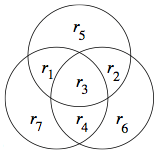
\includegraphics[width=0.2\textwidth]{hamming_code_circles.png}
	\caption{Hamming Code Venn Diagram}
\end{figure}

While the diagram is useful for visualization, a more efficient way to encode a message is to multiply it with the generator matrix \textbf{G}.

$$
\textbf{G} = 
\left(
\begin{array}{ccccccc}
1 & 0 & 0 & 0 & 1 & 0 & 1\\
0 & 1 & 0 & 0 & 1 & 1 & 0\\
0 & 0 & 1 & 0 & 1 & 1 & 1\\
0 & 0 & 0 & 1 & 0 & 1 & 1
\end{array}
\right)
=
\left[
I_4 \vert P^T
\right]
$$
$$
\textbf{H} =
\left(
\begin{array}{ccccccc}
1 & 1 & 1 & 0 & 1 & 0 & 0\\
0 & 1 & 1 & 1 & 0 & 1 & 0\\
1 & 0 & 1 & 1 & 0 & 0 & 1
\end{array}
\right)
=
\left[
-P \vert I_3
\right]
$$

To encode a message \textbf{x} of length 4, we perform $\textbf{G}^T \cdot \textbf{x}$. From the transmitted message \textbf{t}, we first compute the syndrome vector \textbf{z} via $\textbf{z} = \textbf{H} \cdot \textbf{t}$. Based on the results of \textbf{z}, we flip the $i^{th}$ position bit according to the table shown below:

$$
\begin{array}{|c|cccccccc|}
\hline
\text{Syndrome \textbf{z}} 	& 000 & 001 & 010 & 011 & 100 & 101 & 110 & 111\\
\hline
\text{Flip this bit} 		&  -  & r_7 & r_6 & r_4 & r_5 & r_1 & r_2 & r_3\\
\hline
\end{array}
$$

As we send 7 bits for every 4 bits of information, the $(7,4)$ Hamming code attains a rate of $\frac{4}{7}$. Also, since we are able to correct only up to 1 error during transmission, we have a block error whenever $\geq 2$ out of the 7 transmitted bits are corrupted. In a binary symmetric channel with error probability $f$, that translates to a block error rate of $1 - \Pr(\text{No flipped bits}) - \Pr(\text{1 flipped bit}) = 1 - (1-f)^7 - \binom{7}{1}f(1-f)^6$.


\subsection{$(9,5)$ Suggested Code}
In the suggested solutions to the first homework, we are given the following error-correcting code:

\begin{quote}
We encode a string of 5 bits $(k = 5)$ \textbf{s} = $(s_i)_{1 \leq i \leq5}$ into a 9-bit string $(n = 9)$ \textbf{t} = $(t_i)_{1 \leq i \leq 9}$. The first 5 bits of \textbf{t} will be identical to those of \textbf{s}, while the other 4 are parity bits. To choose the parity bits, we take inspiration from inscribing the bits as a cross within a square; parity bits are the sum of the three neighboring bits within the square:
\begin{figure}[H]
	\centering
	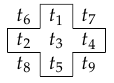
\includegraphics[width=0.2\textwidth]{suggested_diagram.png}
\end{figure}
In other words,\\
$t6 = t1+t2+t3, t7 = t1+t3+t4, t8 = t2+t3+t5, t9 = t3+t4+t5$.
\end{quote}

As per the $(7,4)$ Hamming code, it is more efficient to encode messages using a generator matrix \textbf{G} instead of directly making use of the diagram.

$$
\textbf{G} = 
\left(
\begin{array}{ccccccccc}
1 & 0 & 0 & 0 & 0 & 1 & 1 & 0 & 0\\
0 & 1 & 0 & 0 & 0 & 1 & 0 & 1 & 0\\
0 & 0 & 1 & 0 & 0 & 1 & 1 & 1 & 1\\
0 & 0 & 0 & 1 & 0 & 0 & 1 & 0 & 1\\
0 & 0 & 0 & 0 & 1 & 0 & 0 & 1 & 1
\end{array}
\right)
=
\left[
I_5 \vert P^T
\right]
$$
$$
\textbf{H} =
\left(
\begin{array}{ccccccccc}
1 & 1 & 1 & 0 & 0 & 1 & 0 & 0 & 0\\
1 & 0 & 1 & 1 & 0 & 0 & 1 & 0 & 0\\
0 & 1 & 1 & 0 & 1 & 0 & 0 & 1 & 0\\
0 & 0 & 1 & 1 & 1 & 0 & 0 & 0 & 1
\end{array}
\right)
=
\left[
-P \vert I_4
\right]
$$

To encode a message \textbf{x} of length 5, we perform $\textbf{G}^T \cdot \textbf{x}$. From the transmitted message \textbf{t}, we first compute the syndrome vector \textbf{z} via $\textbf{z} = \textbf{H} \cdot \textbf{t}$. Based on the results of \textbf{z}, we flip the $i^{th}$ position bit according to the table shown below:

$$
\begin{array}{|c|ccccccccccc|}
\hline
\text{Syndrome \textbf{z}} 	& 0000 & 1100 & 1010 & 1111 & 0101 & 0011 & 1000 & 0100 & 0010 & 0001 & \text{Others}\\
\hline
\text{Flip this bit} 		&  -  & t_1 & t_2 & t_3 & t_4 & t_5 & t_6 & t_7 & t_8 & t_9 & \text{Error}\\
\hline
\end{array}
$$

For `Error', we can choose not to flip anything since we will not be able to correct the block anyway. The analysis for this code is similar to that of the (7,4) Hamming code.

As we send 9 bits for every 5 bits of information, the suggested code attains a rate of $\frac{5}{9}$. Also, since we are able to correct only up to 1 error during transmission, we have a block error whenever $\geq 2$ out of the 9 transmitted bits are corrupted. In a binary symmetric channel with error probability $f$, that translates to a block error rate of $1 - \Pr(\text{No flipped bits}) - \Pr(\text{1 flipped bit}) = 1 - (1-f)^9 - \binom{9}{1}f(1-f)^8$.

\subsection{$\mathcal{R}(1,3)$ Reed-Muller Code}
\subsubsection{$\mathcal{R}(r,m)$ Reed-Muller Codes}
Reed-Muller codes are a family of linear error-correcting codes named after Irving S. Reed and David E. Muller. They are usually listed as $\mathcal{R}(r,m)$, where the $r$ represents the order of the code and $m$ represents the $\log_2$ length of the code (i.e. code length = $2^m$).

There are several interesting properties about Reed-Muller Codes\footnote{Source: \url{http://en.wikipedia.org/wiki/Reed–Muller_code}}. For instance, $\mathcal{R}(0,m)$ codes are repetition codes, while $\mathcal{R}(1,m)$ codes are parity check codes. It is also known that a $\mathcal{R}(r,m)$ Reed Muller code has minimum distance $d_{min} = 2^{m-r}$.

Before we explain how a generator matrix for a general $\mathcal{R}(r,m)$ Reed-Muller code is formed, let us first define what it means to be a order $r$ Reed-Muller code, and how does $m$ come into the picture.

In a $\mathcal{R}(r,m)$ Reed-Muller code, we have $m$ variables $x_1, x_2, ... , x_m$. Let $M = \{x_1, x_2, ... , x_m\}$ Then, within the power set $\mathcal{P}(M)$ of $M$, we consider only the subsets of up to size $r$. That is to say, out of all the subsets in $\mathcal{P}(M)$, we look at $\sum_{k=0}^{r} \binom{m}{k}$ subsets in total.

Now, when we construct the [$\sum_{k=0}^{r} \binom{m}{k}$]x[$2^m$] generator matrix for the $\mathcal{R}(r,m)$ Reed-Muller code as follows:
\begin{figure}[H]
	\centering
	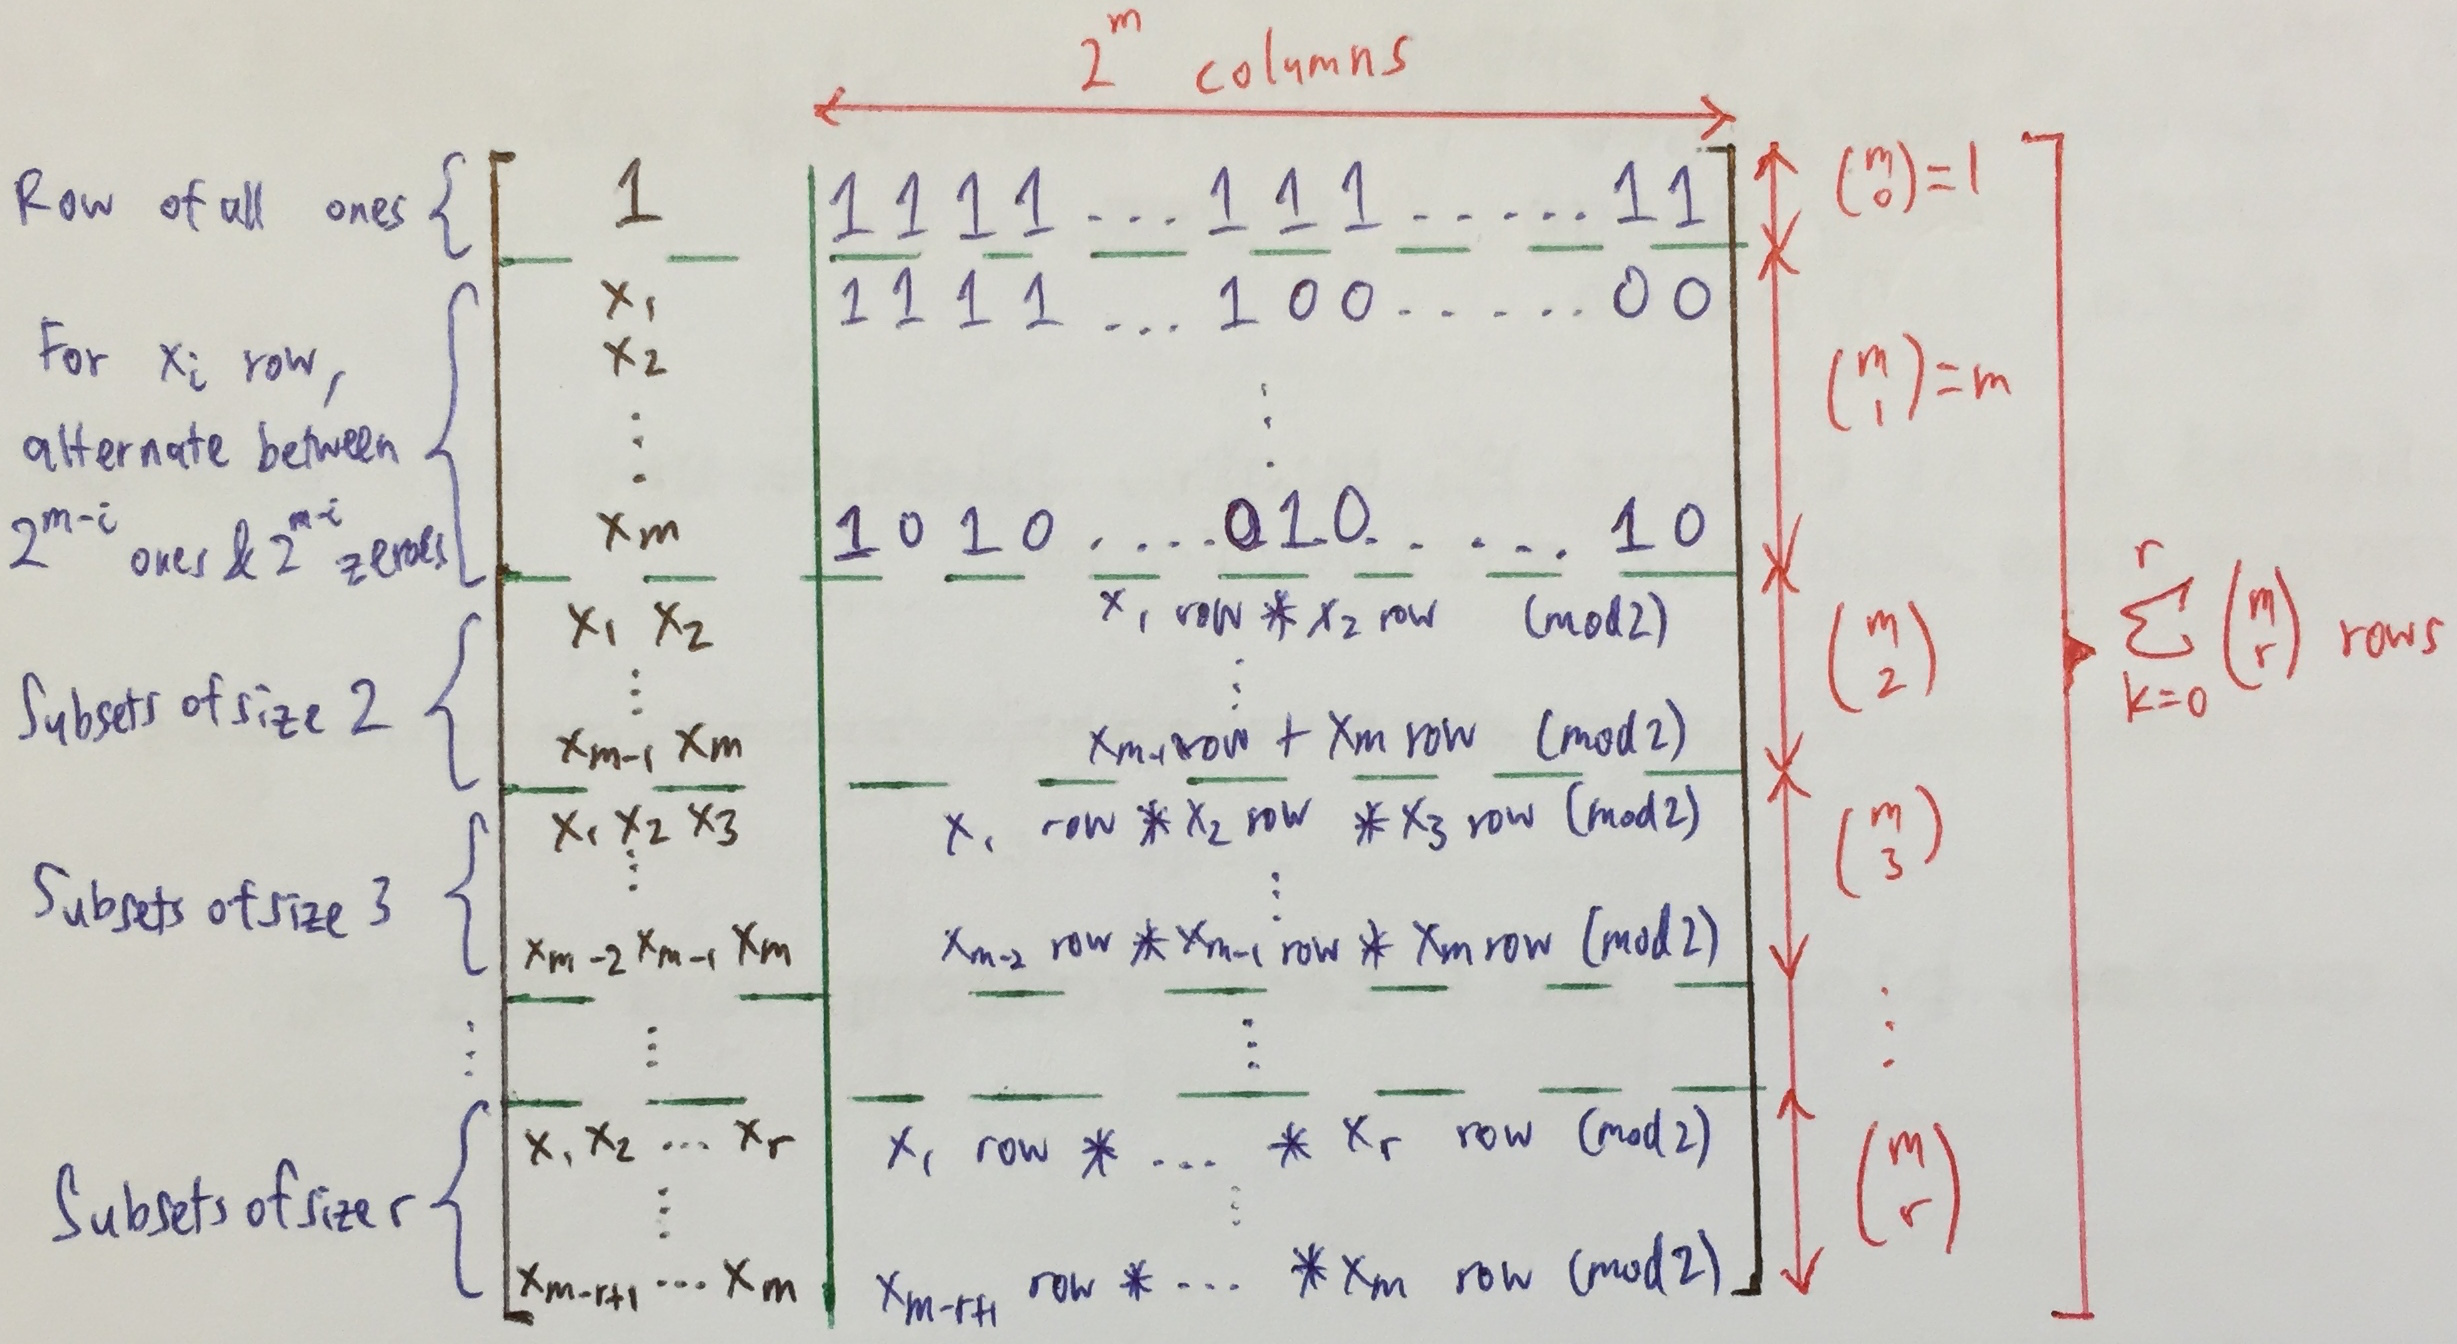
\includegraphics[width=\textwidth]{reedmuller_diagram.jpg}
\end{figure}

Note that $\forall a, b \in \{0,1\}, a * b = 1$ if $a = b = 1$, and $a * b = 0$ otherwise.\footnote{One can think of $a * b$ as ``$a$ (logical AND) $b$''.}

For example, when $r = 2, m = 3$, we have $x_1, x_2, x_3$ and we only consider the subsets $\emptyset, \{x_1\}, \{x_2\}, \{x_3\}, \{x_1, x_2\}, \{x_1, x_3\}, \{x_2, x_3\}$. We obtain the following generator matrix:

$$
\left[
\begin{array}{c|cccccccc}
\textbf{1} 			& 1 & 1 & 1 & 1 & 1 & 1 & 1 & 1\\
\textbf{$x_1$} 		& 1 & 1 & 1 & 1 & 0 & 0 & 0 & 0\\
\textbf{$x_2$} 		& 1 & 1 & 0 & 0 & 1 & 1 & 0 & 0\\
\textbf{$x_3$} 		& 1 & 0 & 1 & 0 & 1 & 0 & 1 & 0\\
\textbf{$x_1x_2$} 	& 1 & 1 & 0 & 0 & 0 & 0 & 0 & 0\\
\textbf{$x_1x_3$} 	& 1 & 0 & 1 & 0 & 0 & 0 & 0 & 0\\
\textbf{$x_2x_3$} 	& 1 & 0 & 0 & 0 & 1 & 0 & 0 & 0
\end{array}
\right]
$$

To encode a message \textbf{x} of length $\sum_{k=0}^{r} \binom{m}{k}$, we perform $\textbf{G}^T \cdot \textbf{x}$. While encoding Reed-Muller codes are as easy as encoding Hamming codes, it is less trivial to decode Reed-Muller codes. The high level idea of the decoding process is majority decoding. For the exact details on the general decoding of Reed-Muller codes, we refer readers to the references cited at the end of the report. We will only go through the simple example of decoding our $\mathcal{R}(1,3)$ Reed-Muller code.

% Let us walk through the steps of decoding a general $\mathcal{R}(r,m)$ Reed-Muller code.

% To begin, we need to consider the characteristic vectors of each row (except the \textbf{1} row). To obtain the characteristic vectors for the row $x_ix_j...x_k$, we first consider the set $C = M \setminus \{x_i,x_j,...,x_k\}$. We then consider $2^C$ vectors obtained in the following manner:

% \begin{enumerate}
% \item Line up the elements in $C$, say $x_\alpha, x_\beta, ... , x_\gamma$.
% \item Consider the set of $2^|C|$ strings $00...0$, $00...1$ all the way to $11...1$
% \item Map each of these strings to a multiplication of elements in $C$ by replacing the $i^{th}$ character in the string with $x_i$ if it is ``1'' and $\overline{x_i}$ if it is ``0''.
% \item Denote the resultant set of characteristic vectors as $CV$
% \end{enumerate}

% Now, given a transmitted message \textbf{t}, do the following for every row $R$ (except the \textbf{1} row):

% \begin{enumerate}
% \item Take the dot product of \textbf{t} with every element in $CV$, modulo 2. We should obtain a set of ``1'' and ``0''.
% \item If we have more ``1'' than ``0'', return ``1'' as the coefficient for the row $R$. Otherwise, return ``0''
% \end{enumerate}

% After this step, we should have 

\subsubsection{$\mathcal{R}(1,3)$ Reed-Muller Code}
In this project, we investigate a specific instance of the $\mathcal{R}(1,3)$ Reed-Muller code. Using the construction mentioned above, we obtain the following $4 \times 8$ generator matrix \textbf{G}.

$$
\textbf{G} = 
\left[
\begin{array}{c|cccccccc}
\textbf{1} 			& 1 & 1 & 1 & 1 & 1 & 1 & 1 & 1\\
\textbf{$x_1$} 		& 1 & 1 & 1 & 1 & 0 & 0 & 0 & 0\\
\textbf{$x_2$} 		& 1 & 1 & 0 & 0 & 1 & 1 & 0 & 0\\
\textbf{$x_3$} 		& 1 & 0 & 1 & 0 & 1 & 0 & 1 & 0
\end{array}
\right]
$$

To decode, we first calculate the characteristic vectors of each row:
\begin{itemize}
\item Characteristic vectors of $CV_{x_3} = \{x_1x_2, x_1\overline{x_2}, \overline{x_1}x_2, \overline{x_1}\overline{x_2}\}$
\item Characteristic vectors of $CV_{x_2} = \{x_1x_3, x_1\overline{x_3}, \overline{x_1}x_3, \overline{x_1}\overline{x_3}\}$
\item Characteristic vectors of $CV_{x_1} = \{x_2x_3, x_2\overline{x_3}, \overline{x_2}x_3, \overline{x_2}\overline{x_3}\}$
\end{itemize}
After that, we find the dot product (modulo 2) between the transmitted vector \textbf{t} with each of these characteristic vectors. This process will give us 4 values in $\{0,1\}$. We say the cofficient of the corresponding row $c_i$ is `1' if we have more `1's than `0's out of the 4 values, and `0' otherwise.

At the end of the previous step, we would have the coefficients for the rows $x_1, x_2, x_3$. To calculate the coefficient for the row \textbf{1}, we compute $c_1x_1 + c_2x_2 + c_3x_3 + \textbf{t}$ (modulo 2). We say the cofficient of $c_0$ is `1' if we have more `1's than `0's out of the resultant vector, and `0' otherwise.

Lastly, we output the received message as $(c_0, c_1, c_2, c_3)$.

To make things concrete, let us step through the decoding of the following transmitted message \textbf{t = 01010110}.

Recall that:
$$
\begin{array}{ccc}
\textbf{1} & = &11111111\\
x_1 & = & 11110000\\
x_2 & = & 11001100\\
x_3 & = &10101010
\end{array}
$$

Then,
$$
\begin{array}{ccccc}
CV_{x_3} & = & \{x_1x_2, x_1\overline{x_2}, \overline{x_1}x_2, \overline{x_1}\overline{x_2}\} & = & \{11000000, 00110000, 00001100, 00000011\}\\
CV_{x_2} & = & \{x_1x_3, x_1\overline{x_3}, \overline{x_1}x_3, \overline{x_1}\overline{x_3}\} & = & \{10100000, 01010000, 00001010, 00000101\}\\
CV_{x_1} & = & \{x_2x_3, x_2\overline{x_3}, \overline{x_2}x_3, \overline{x_2}\overline{x_3}\} & = & \{10001000, 01000100, 00100010, 00010001\}
\end{array}
$$

We can check that the dot products with \textbf{t} give us:
$$
\begin{array}{ccc}
\textbf{t} \cdot CV_{x_3} & = & \{1, 1, 1, 1\}\\
\textbf{t} \cdot CV_{x_2} & = & \{0, 0, 1, 1\}\\
\textbf{t} \cdot CV_{x_1} & = & \{0, 0, 1, 1\}
\end{array}
$$

So, $c_3 = 1, c_2 = 0, c_1 = 0$. Then $c_1x_1 + c_2x_2 + c_3x_3 + \textbf{t}$ (modulo 2) = $11111100$. So $c_0 = 1$. Hence, the decoded message is \textbf{1001}.

Since the minimum distance of the $\mathcal{R}(1,3)$ Reed-Muller code is $d_{min} = 2^{m-r} = 2^{3-1} = 4$, the maximum number of errors that it can correct is $t = \lfloor (d_{min}-1)/2 \rfloor = \lfloor (4-1)/2 \rfloor = \lfloor 1.5 \rfloor = 1$.

As we send 8 bits for every 4 bits of information, the $\mathcal{R}(1,3)$ Reed-Muller code attains a rate of $\frac{4}{8}$. Also, since we are able to correct only up to 1 error during transmission, we have a block error whenever $\geq 2$ out of the 8 transmitted bits are corrupted. In a binary symmetric channel with error probability $f$, that translates to a block error rate of $1 - \Pr(\text{No flipped bits}) - \Pr(\text{1 flipped bit}) = 1 - (1-f)^8 - \binom{8}{1}f(1-f)^7$.

\section{Implementation and experiments}
\subsection{Implementation}
We used Python and the numpy package in the implementation of our project. This choice was due to the fact that our error-correcting codes were linear codes and we could make use of numpy's various useful matrix methods.

To speed up simulation, we treat the entire file as a single matrix instead of a list of vectors. For a $(b, a)$ error-correcting code\footnote{We send $b$ bits to convey $a$ bits of information.}, we break up the input file of $N$ bits into a $a \times \lceil \frac{N}{a} \rceil$ matrix\footnote{We pad with 0's if necessary.}. After that, we encode the entire message matrix via a single matrix multiplication with \textbf{G} to obtain a $b \times \lceil \frac{N}{a} \rceil$ encoded matrix. To simulate a binary symmetric channel with error probability $f$, we simply generate a random noise $\{0,1\}$ matrix ($1$ with probability $f$) of size $b \times \lceil \frac{N}{a} \rceil$. Lastly, perform the $XOR$ operation with the noise and encoded matrices to obtain our transmitted matrix, from which we decode the message from.

\subsection{Dataset}
We tested our error-correcting codes on 2 types of datasets:
\begin{itemize}
\item 1000 500KB files of generated using Python's \textsc{os.urandom}
\item Some images to have a visual comparison
\end{itemize}

\subsection{Results}
Let us look at the summary of some theoretical properties about each of our 3 error-correcting codes. From the above sections, our \textbf{min\_dist.py} script, and the equation for maximum error correction $t = \lfloor (d_{min}-1)/2 \rfloor$, we get the following table\footnote{$BSC_f$ means a binary symmetric channel with bit error probability $f$}:
$$
\begin{array}{|c||c|c|c|c|}
\hline
\text{Code} & \text{Rate} & d_{min} & t & \text{Block error rate on } BSC_f\\
\hline
(7,4) \text{Hamming Code} & 4/7 & 3 & 1 & 1 - (1-f)^7 - \binom{7}{1}f(1-f)^6\\
(9,5) \text{ Suggested Code } & 5/9 & 3 & 1 & 1 - (1-f)^9 - \binom{9}{1}f(1-f)^8\\
\mathcal{R}(1,3) \text{ Reed-Muller Code } & 4/8 & 4 & 1 & 1 - (1-f)^8 - \binom{8}{1}f(1-f)^7\\
\hline
\end{array}
$$
Let us consider the block error rates of our codes on a few values of $f$ (rounded to 3 decimal places)\footnote{Obtained using our script \textbf{block\_error.py}.}.
$$
\begin{array}{|c||c|c|c|c|c|c|c|c|c|}
\hline
f & \frac{1}{2} & \frac{1}{3} & \frac{1}{4} & \frac{1}{5} & \frac{1}{6} & \frac{1}{7} & \frac{1}{8} & \frac{1}{9} & \frac{1}{10}\\
\hline
(7,4) \text{Hamming Code} & 0.938 & 0.737 & 0.555 & 0.423 & 0.33 & 0.264 &  0.215 & 0.178 & 0.15\\
(9,5) \text{ Suggested Code } & 0.98 & 0.857 & 0.7 & 0.564 & 0.457 & 0.376 & 0.313 & 0.264 & 0.225\\
\mathcal{R}(1,3) \text{ Reed-Muller Code } &0.965 & 0.805 & 0.633 & 0.497 & 0.395 & 0.32 & 0.264 & 0.221 & 0.187\\
\hline
\end{array}
$$
We see that the $(7,4)$ Hamming Code seems to perform the best while the suggested $(9,5)$ code is the worst of the 3. We verify this with empirical results. First we generated 1000 500KB files of bytes using Python's \textsc{os.urandom}. For each of the error-correcting schemes, we encode the files, simulate passing through a noisy $BSC_f$ and then decode it. The following table shows the \textit{mean block error rates} over 1000 files.
%$$
%\begin{array}{|c||c|c|c|c|c|c|c|c|c|}
%\hline
%f & \frac{1}{2} & \frac{1}{3} & \frac{1}{4} & \frac{1}{5} & \frac{1}{6} & \frac{1}{7} & \frac{1}{8} & \frac{1}{9} & \frac{1}{10}\\
%\hline
%(7,4) \text{Hamming Code} & 0.996 & 0.961 & 0.9 & 0.832 & 0.767 & 0.709 & 0.656 & 0.61 & 0.57\\
%(9,5) \text{ Suggested Code } & 0.996 & 0.961 & 0.9 & 0.832 & 0.767 & 0.709 & 0.656 & 0.61 & 0.57\\
%\mathcal{R}(1,3) \text{ Reed-Muller Code } & 0.996 & 0.938 & 0.819 & 0.69 & 0.575 & 0.481 & 0.405 & 0.344 & 0.295\\
%\hline
%\end{array}
%$$
$$
\begin{array}{|c||c|c|c|c|c|c|c|c|c|}
\hline
f & \frac{1}{2} & \frac{1}{3} & \frac{1}{4} & \frac{1}{5} & \frac{1}{6} & \frac{1}{7} & \frac{1}{8} & \frac{1}{9} & \frac{1}{10}\\
\hline
(7,4) \text{Hamming Code} & 0.938 & 0.802 & 0.684 & 0.590 & 0.518 & 0.460 & 0.414 & 0.376 & 0.344\\
(9,5) \text{ Suggested Code } & 0.969 & 0.868 & 0.763 & 0.672 & 0.598 & 0.537 & 0.487 & 0.445 & 0.410\\
\mathcal{R}(1,3) \text{ Reed-Muller Code } & 0.937 & 0.751 & 0.575 & 0.443 & 0.348 & 0.279 & 0.228 & 0.190 & 0.160\\
\hline
\end{array}
$$


\begin{figure}[H]
	\centering
	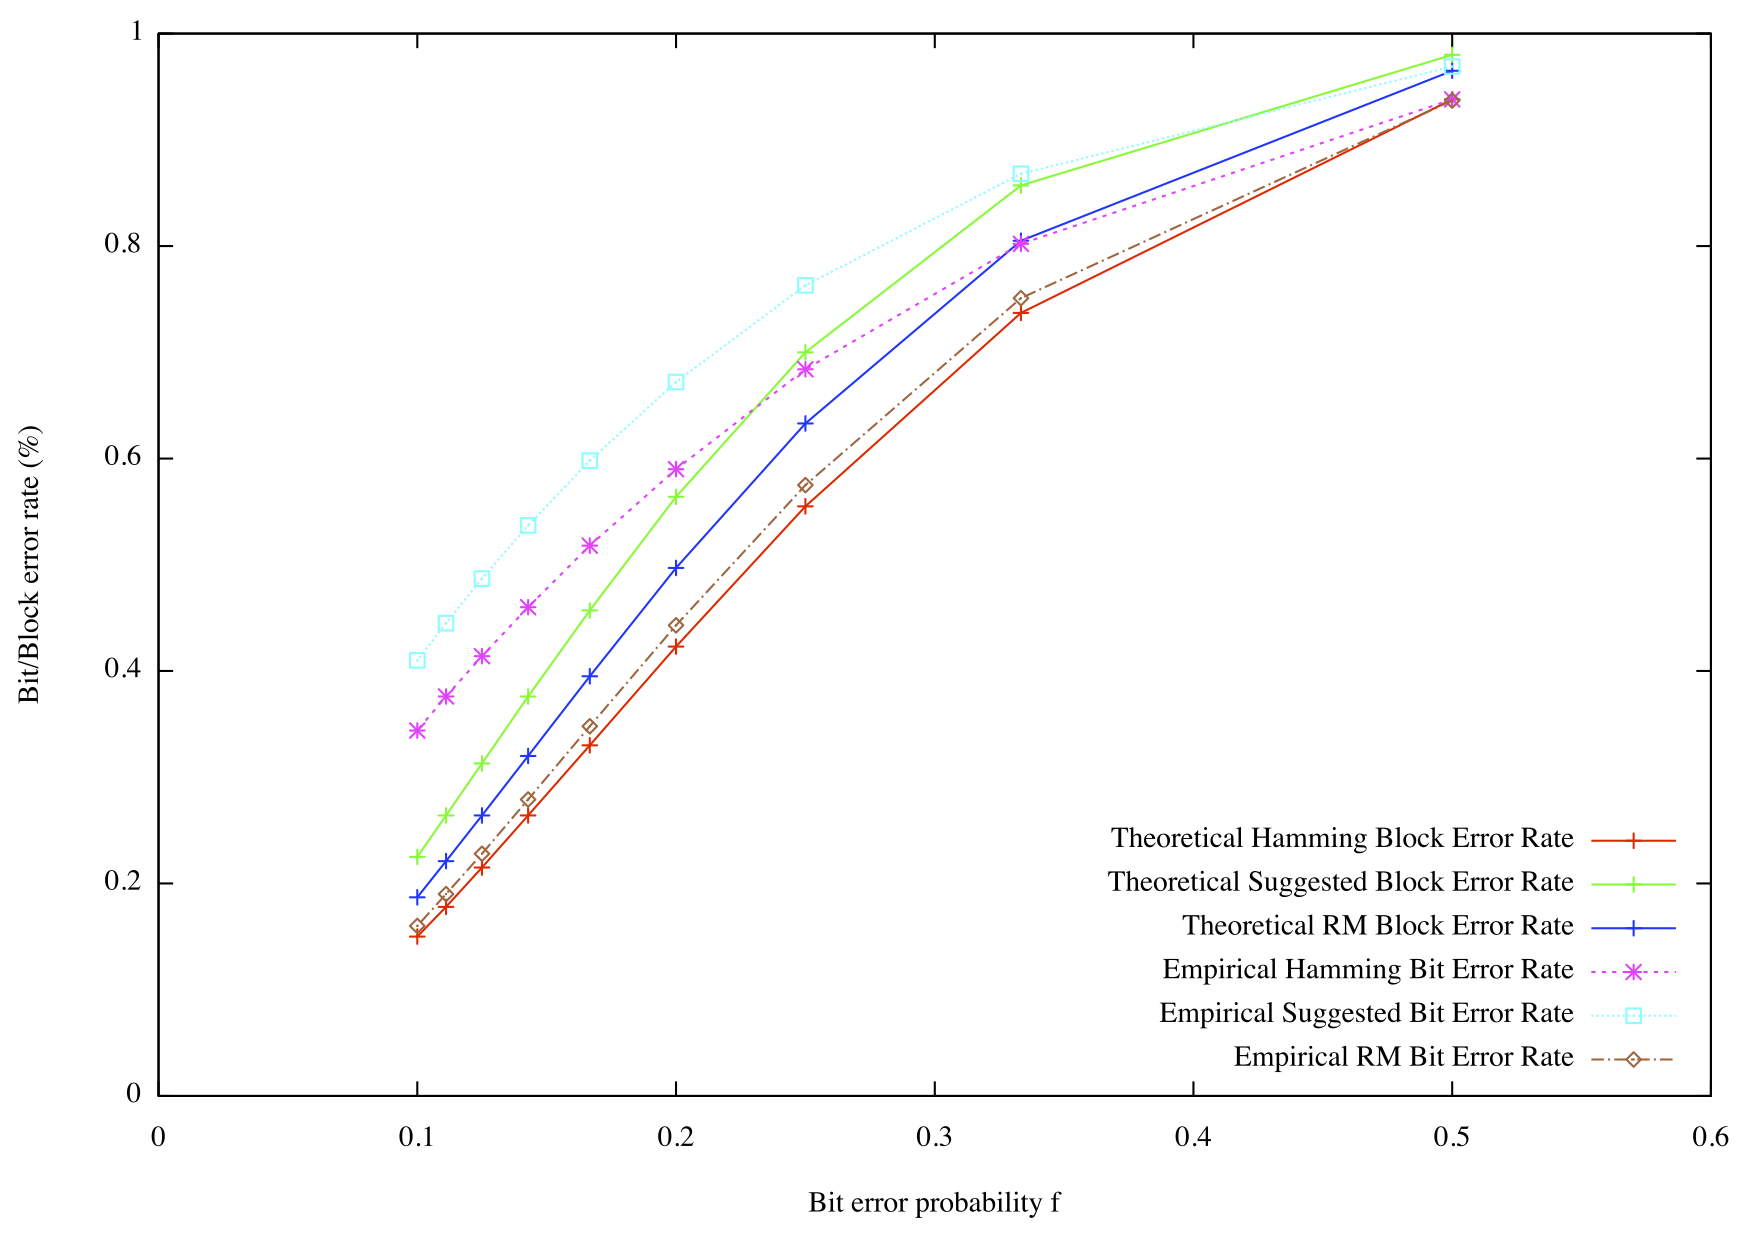
\includegraphics[width=\textwidth]{results.png}
	\caption{Relationship between $f$ and bit/block error rates, for $f = \{\frac{1}{2}, \frac{1}{3}, ... , \frac{1}{10}\}$}
\end{figure}

The empirical results support the general trends described by the theoretical analysis. However, it is interesting to observe that the Reed-Muller code performs empirically better than the Hamming code despite the latter having a lower theoretical block error rate.

We conclude the report with image simulations. This is to visualize the difference in performance of the 3 error-correcting codes. We enlist the help of 2 different images - A Pokemon image\footnote{Source: \url{http://pt.todoprogramas.com/photos/2009/2/1024.877.273.1a.500.jpg}} and a smiley face\footnote{Source: \url{http://www.imgion.com/images/01/Blurred-smiley.gif}}. The images are converted to .ppm format before the simulation is ran\footnote{We fix any corrupted .ppm headers using \textit{dd if=$<$original\_image$>$ of=$<$new\_image$>$ bs=15 count=1 conv=notrunc}}. The image tilings shown below are ordered in the following manner:

\begin{table}[H]
\centering
\begin{tabular}{|c|c|}
\hline
Original Image & Hamming Code\\
\hline
Suggested Code & Reed-Muller Code\\
\hline
\end{tabular}
\end{table}

\begin{figure}[H]
	\centering
	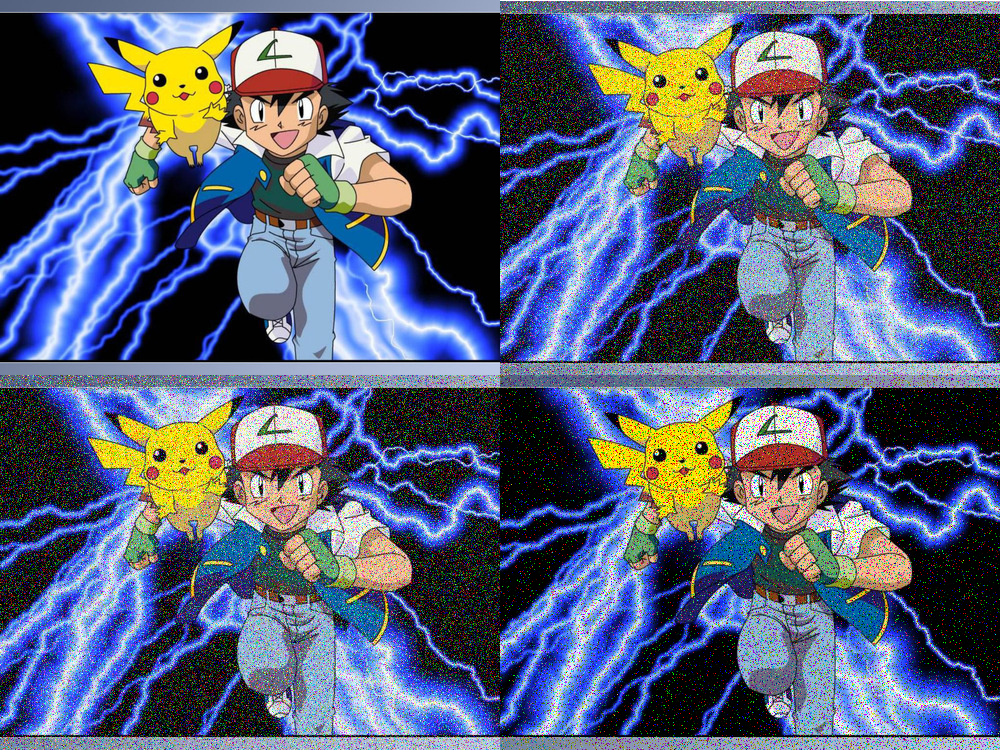
\includegraphics[width=0.8\textwidth]{pokemon_tile10.png}
	
\includegraphics[width=0.8\textwidth]{smiley_tile10.png}
	\caption{Simulation with $f = \frac{1}{10}$}
\end{figure}
\begin{figure}[H]
	\centering
	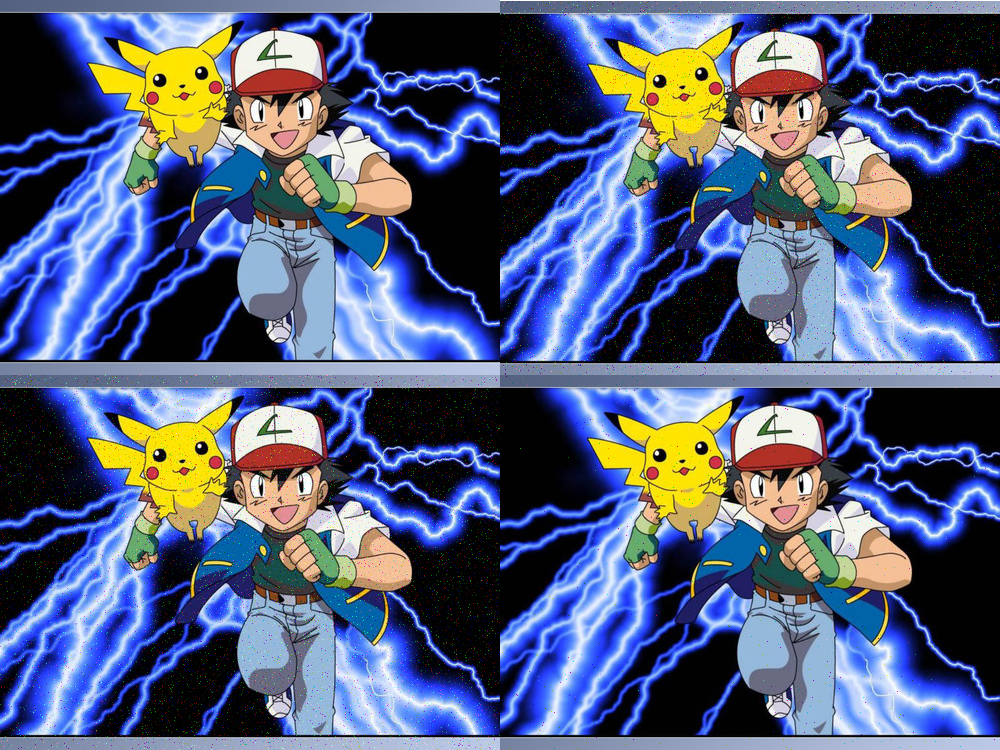
\includegraphics[width=0.8\textwidth]{pokemon_tile100.png}
	
\includegraphics[width=0.8\textwidth]{smiley_tile100.png}
	\caption{Simulation with $f = \frac{1}{100}$}
\end{figure}

\section{References}
Source code is available on Github: \url{https://github.com/sozos/CodingSchemes}

David J.C. MacKay. (2003). \textit{Information Theory, Inference, and Learning Algorithms}. Cambridge, UK: Cambridge University Press

Ben Cooke. \textit{Reed-Muller Error Correcting Codes}. MIT Undergraduate Journal of Mathematics. Retrived from \url{http://www-math.mit.edu/phase2/UJM/vol1/COOKE7FF.PDF}

Irving S. Reed. (1954). A class of multiple-error-correcting codes and the decoding scheme. \textit{IEEE Trans. on Information Theory}, 4:38-49.

% End content
\end{document}